% \documentclass{article}
\documentclass[a4paper]{article}
\usepackage{/Users/mariachrysafis/Documents/Schoolwork/18.650/chrysafis}
\graphicspath{ {/} }
\begin{document}
\section{probability review}
\begin{Exercise}
	Let $X$ be a random variable taking values between $0$ and $\pi$ with pdf given by $f(x) = c\sin(x), x \in [0, \pi].$ What is the value of $c$?
\end{Exercise}
\begin{Solution}
	Since the integral of the pdf is always $1$ (by definition),
	\begin{align*}
		1 = \int_{0}^{\pi} f(x) \dd{x} = \int_{0}^{\pi} c \sin x \dd{x} = -c \Big|_{0}^{\pi} \cos x = -c (\cos \pi - \cos 0) = -c (-2) = 2c. 
	\end{align*}
	And so, $2c = 1$ and $c = \frac{1}{2}$. $\boxed{B}$.
\end{Solution}
\begin{Exercise}
	What is $\mathbb{E}[X]$?
\end{Exercise}
\begin{Solution}
	By the definition of expectation, 
	\begin{align*}
		\mathbb{E}[X] = \int_{0}^{\pi} x f(x) \dd{x} = \int_0^{\pi} c x \sin x \dd{x} = c \Big|_0^{\pi} \left( \sin x - x \cos x \right) = c (-\pi \cos \pi + \sin \pi - 0 \cos 0 + \sin 0) = \pi c.
	\end{align*}
	We know from the previous problem that $c = \frac{1}{2}$, so $\mathbb{E}[X] = \frac{\pi}{2}.$ $\boxed{A}$.
\end{Solution}
\begin{Exercise}
	Let $X$ be a Gaussian random variable with mean $\mu >0$ and variance $\mu^2$. What is $\mathbb{E}[X]$?
\end{Exercise}
\begin{Solution}
	The mean, that is $\mathbb{E}[X]$, is $\mu$ by definition. $\boxed{B}$.
\end{Solution}
\begin{Exercise}
	What is $\mathbb{E}[X^2]$?
\end{Exercise}
\begin{Solution}
	By definition of variance,
	\begin{align*}
		\mu^2 = \text{Var}[X] = \mathbb{E}[X^2] - \mathbb{E}[X]^2 = \mathbb{E}[X^2] - \mu^2,
	\end{align*}
	so $\mathbb{E}[X^2] = 2 \mu^2.$ $\boxed{C}$.
\end{Solution}
\begin{Exercise}
	What is $\mathbb{E}[X^3]$?
\end{Exercise}
\begin{Solution}
	Using the binomial theorem,
	\begin{align*}
		\mathbb{E}[X^3] &= \mathbb{E}[((X - \mu) + \mu)^3] 
			     \\ &= \mathbb{E}[(X - \mu)^3] + 3 \mathbb{E}[(X - \mu)^2 \mu] + 3\mathbb{E}[(X - \mu)\mu^2] + \mathbb{E}[\mu^3]
			     \\ &= 3 \mu \mathbb{E}[(X - \mu)^2] + \mu^3.
	\end{align*}
	Since $X - \mu$ is a Gaussian random variable with mean $0$ and variance $\mu^2$, $\mathbb{E}[(X - \mu)^2] = \mu^2$, 
	\begin{align*}
		\mathbb{E}[X^3] = 3 \mu^3 + \mu^ = 4 \mu^3.3
	\end{align*}
	$\boxed{C}$.
\end{Solution}
\begin{Exercise}
	What is $\text{Var}[X^2]$?
\end{Exercise}
\begin{Solution}
	For a normal random variable with mean $\mu$ and standard deviation $\sigma$, $\mathbb{E}[X^4] = 3 \sigma^4 + 6 \mu^2 \sigma^2 + \mu^4$. Since our mean and standard deviation are both $\mu$ in this case, $\mathbb{E}[X^4] = 10 \mu^4.$ Using this, 
	\begin{align*}
		\text{Var}[X^2] &= \mathbb{E}[X^4]- \mathbb{E}[X^2]^2
			     \\ &= 10 \mu^4 - (2 \mu^2)^2
			     \\ &= 6 \mu^4.
	\end{align*}
	$\boxed{B}$.
\end{Solution}
\begin{Exercise}
	What is $\mathbb{P}[X > 0]$ in terms of the CDF $\Phi$ of the standard Gaussian distribution?
\end{Exercise}
\begin{Solution}
	By definition of the cdf, $$\mathbb{P}[X > 0] = \mathbb{P} \left[ \frac{X - \mu}{\sigma} > -\frac{\mu}{\sigma} \right] = \mathbb{P} \left[ \frac{X - \mu}{\sigma} > -1 \right] = \mathbb{P} \left[ \frac{X - \mu}{\sigma} < \right] = \Phi(1).$$
	$\boxed{B}$.
\end{Solution}
\begin{Exercise}
	Let $X$ be a random variable such that
	\begin{align*}
		X = \begin{cases}
			1 & \text{with probability } p \\
			-1 & \text{with probability } 1- p
		\end{cases}
	\end{align*}
	for some $p \in [0, 1]$. What is $\mathbb{E}[X]$?
\end{Exercise}
\begin{Solution}
	Routine algebra shows that $\mathbb{E}[X] = 1 \cdot p + (-1) \cdot (1 - p) = -1 + 2p.$ $\boxed{D}$.
\end{Solution}
\begin{Exercise}
	What is $\text{Var}[X]$?
\end{Exercise}
\begin{Solution}
	The variance of $X$ is $\mathbb{E}[X^2] - \mathbb{E}[X]^2 = 1 - (1 - 2p)^2 = 4p - 4p^2 = 4p (1 - p).$ $\boxed{C}$.
\end{Solution}
\begin{Exercise}
	For what $p$ is $\text{Var}[X]$ maximized?
\end{Exercise}
\begin{Solution}
	We know from the previous problem that $\text{Var}[X] = 4p - 4p^2$, which has derivative $4 - 8p$. The variance is maximized when that derivative is $0$, so when $4 - 8p = 0 \Longrightarrow p = \frac{1}{2}.$ $\boxed{C}$.
\end{Solution}
\begin{Exercise}
	What is $\mathbb{E}[X^k]$?
\end{Exercise}
\begin{Solution}
	The expected value is $\mathbb{E}[X^k] = 1^k \cdot p + (-1)^k \cdot (1 - p) = p + (-1)^k \cdot (1 - p)$. $\boxed{D}$.
\end{Solution}
\begin{Exercise}
	Let $X$ and $Y$ be two independent standard Gaussian random variables. What is $\mathbb{E}[X^2Y]$?
\end{Exercise}
\begin{Solution}
	Since $X$ and $Y$ are independent, $\mathbb{E}[X^2Y] = \mathbb{E}[X^2] \cdot \mathbb{E}[Y] = 0.$ $\boxed{A}$.
\end{Solution}
\begin{Exercise}
	What is $\text{Var}(X + Y)$?
\end{Exercise}
\begin{Solution}
	Since $X$ and $Y$ are independent, $\text{Var}[X + Y] = \text{Var}[X] + \text{Var}[Y] = 1 + 1 = 2.$ $\boxed{C}$.
\end{Solution}
\begin{Exercise}
	What is $\text{Var}[XY]$?
\end{Exercise}
\begin{Solution}
	The variance is $\text{Var}[XY] = \mathbb{E}[(XY)^2] - \mathbb{E}[XY]^2 = \mathbb{E}[X^2] \mathbb{E}[Y^2] = 1.$ $\boxed{B}$.
\end{Solution}
\begin{Exercise}
	What is $\text{Cov}[X, X + Y]$?
\end{Exercise}
\begin{Solution}
	The covariance is $\text{Cov}[X, X + Y] = \text{Cov}[X, X] + \text{Cov}[X, Y] = 1 + 0 = 1.$ $\boxed{B}$.
\end{Solution}
\begin{Exercise}
	What is $\text{Cov}[X, XY]$?
\end{Exercise}
\begin{Solution}
	The covariance is $\text{Cov}[X, XY] = \mathbb{E}[X^2Y] - \mathbb{E}[X] \mathbb{E}[XY] = 0.$ $\boxed{A}$.
\end{Solution}
\begin{Exercise}
\end{Exercise}
\begin{Exercise}
\end{Exercise}
\begin{Exercise}
	Let$X_1, \ldots X_n$ be i.i.d. with mean $\mu$ and variance $\sigma^2$. What is $\mathbb{E}\left[\sum_{i = 1}^n X_i\right]$?
\end{Exercise}
\begin{Solution}
	By linearity of expectation,
	\begin{align*}
		\mathbb{E} \left[ \sum_{i = 1}^{n} X_i \right] &= \sum_{i = 1}^{n} \mathbb{E}[X_i] = n \mu.
	\end{align*}
	$\boxed{C}$.
\end{Solution}
\begin{Exercise}
	What is $\text{Var}[\sum_{i = 1}^{n} X_i]$?
\end{Exercise}
\begin{Solution}
	Since each of the $X_i$s are independent,
	\begin{align*}
		\text{Var}\left[ \sum_{i = 1}^{n} X_i \right] = \sum_{i = 1}^{n} \text{Var}[X_i] = n \sigma^2.
	\end{align*}
	$\boxed{B}$.
\end{Solution}
\begin{Exercise}
	What is $\mathbb{E}[(\sum_{i = 1}^{n} X_i)^2]$?
\end{Exercise}
\begin{Solution}
	Let $Y = \sum_{i = 1}^{n} X_i$. Then,
	\begin{align*}
		n\sigma^2 = \text{Var}[Y] = \mathbb{E}[Y^2] - \mathbb{E}[Y]^2 = \mathbb{E}[Y^2] - (n \mu)^2,
	\end{align*}
	so $\mathbb{E}[Y^2] = n^2 \mu^2 + n \sigma^2.$ $\boxed{D}$.
\end{Solution}
\begin{Exercise}
	What is $\text{Var}\left[\frac{1}{n} \sum_{i = 1}^{n} X_i \right]$?
\end{Exercise}
\begin{Solution}
	Since $\text{Var}[aX] = a^2 \text{Var}[X]$,
	\begin{align*}
		\text{Var} \left[ \frac{1}{n} \sum_{i = 1}^{n} X_i \right] = \frac{1}{n^2}\text{Var} \left[ \sum_{i = 1}^{n} X_i \right] = \frac{n \sigma^2}{n^2} = \frac{\sigma^2}{n}.
	\end{align*}
	$\boxed{B}$.
\end{Solution}
\section{new concepts}
\begin{Exercise}
	Let $X_n \sim \text{Unif}(-1/n, 1/n)$ and let $X$ be a random variable such that $\mathbb{P}[X = 0] = 1.$
	\begin{itemize}
		\item[1.] Compute and draw the CDF $F_n(x)$ and $F(x)$ of $X_n$ and $X$ respectively.
		\item[2.] Does $X_n \xrightarrow[]{P} X$? (prove or disprove)
		\item[3.] Does $X_n \rightsquigarrow X$ (prove or disprove)
	\end{itemize}
\end{Exercise}
\begin{Solution}
	\begin{itemize}
		\item[1.] The CDF of $X$ is \begin{align*} F(x) = 
				\begin{cases}
					0 & x < 0 \\ 
					1 & x \ge 0
				\end{cases}
			\end{align*}
			and the CDF of $X_n$ is
			\begin{align*}
				F_n(x) = \begin{cases}
					0 & x < -\frac{1}{n} \\
					\frac{nt + 1}{2} & -\frac{1}{n} \le \frac{1}{n} \\
					1 & x> \frac{1}{n}
				\end{cases}.
			\end{align*}
		\begin{figure}[t]
			\centering
			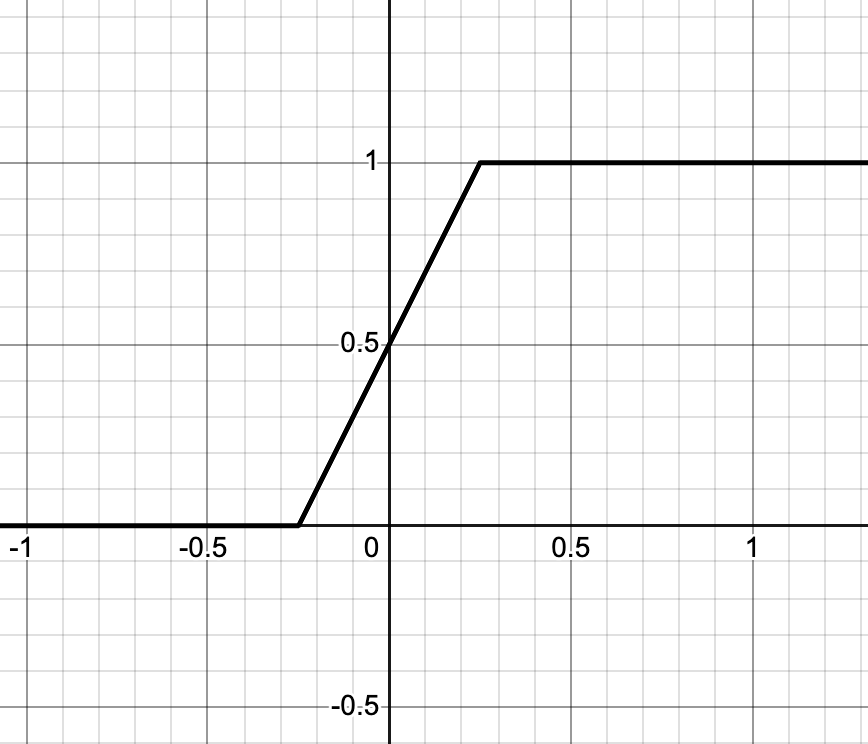
\includegraphics[scale=0.5]{f1}
			\caption{This is the cdf for $X_n$, when $n = 4$.}
		\end{figure}
		\begin{figure}[t]
			\centering
			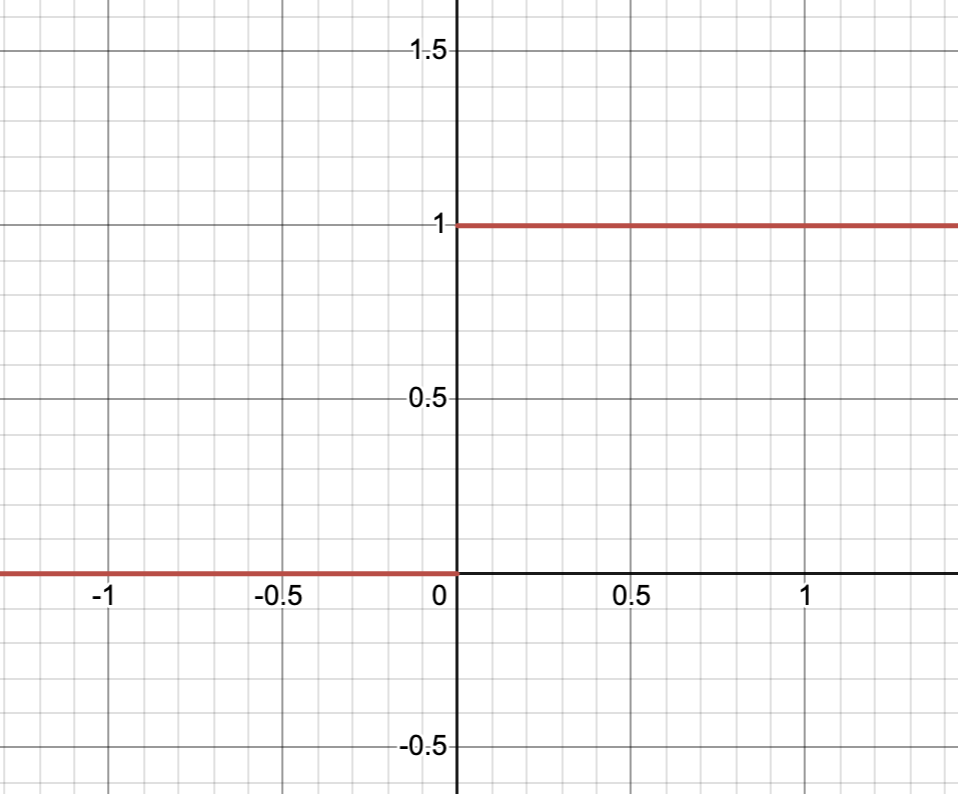
\includegraphics[scale=0.5]{f2}
			\caption{This is the cdf for $X$.}
		\end{figure}
		\item[2.] We know that for all $\epsilon$,
			\begin{align*}
				\mathbb{P}[|X_n - X| > \epsilon] = \mathbb{P}[|X_n| > \epsilon] = 1 - \mathbb{P}[|X_n| \le \epsilon] = 1 - \text{min} \left( \frac{2 \epsilon}{\frac{2}{n}}, 1 \right) = 1 - \min(n \epsilon, 1).
			\end{align*}
			Therefore,
			\begin{align*}
				\lim_{n \to \infty} \mathbb{P}[|X_n - X| > \epsilon] = \lim_{n \to \infty} 1 - \min(n \epsilon, 1) = 0,
			\end{align*}
			so $X_n$ does converge to $X$ probabilistically.
		\item[3.] The CDF of $X$ is 
			\begin{align*}
				F(t) = \begin{cases}
					0 & x < 0 \\
					1 & x \ge 0
				\end{cases}
			\end{align*}
			and the CDF of $X_n$ is 
			\begin{align*}
				F_n(t) = \begin{cases}
					0 & x < -\frac{1}{n} \\
					\frac{nt + 1}{2} & -\frac{1}{n} \le x \le \frac{1}{n} \\ 
					1 & x > \frac{1}{n}
				\end{cases}.
			\end{align*}
			As $n$ approaches $\infty$, $F_n(t)$ approaches
			\begin{align*}
				F_n(t) = \begin{cases}
					0 & x < 0 \\
					\frac{1}{2} & x = \frac{1}{2} \\
					1 & x = 1
				\end{cases}.
			\end{align*}
			Although $F_n(t)$ and $F(t)$ are not the same functions, they have equal values at all points for which $F$ is continous. Thus, $X_n$ converges to $X$ in distribution. 
	\end{itemize}
\end{Solution}
\begin{Exercise}
Let $X \sim \mathcal{N}(1, 2.25)$. Compute the following probabilities (show your work):
\begin{itemize}
	\item[1.] $\mathbb{P}[X > 1]$
	\item[2.] $\mathbb{P}[|X - 2| \le 1]$
	\item[3.] $\mathbb{P}[|X| < 1]$
	\item[4.] $\mathbb{P}[X^2 - 2X - 1 > 0]$.
\end{itemize}
\end{Exercise}
\begin{Solution}
	\begin{itemize}
		\item[1.] Since $X$ is normally distributed around $1$, by symmetry, $\mathbb{P}[X > 1] = 0.5.$ 
		\item[2.] We know that $\mathbb{P}[|X - 2| \le 1] = \mathbb{P}[1 \le X \le 3]$. If we let $Y$ be $\frac{X - \mu}{\sigma} = \frac{X - 1}{1.5}$, then we can rewrite this as $\mathbb{P}\left[0 \le Y \le \frac{4}{3}\right]$. Since $Y$ is standard normal, we can now reference the standard normal table, which tells us that $\mathbb{P}\left[Y \le \frac{4}{3}\right] \approx 0.9082$ and $\mathbb{P}\left[Y \le 0\right] = 0.5$, so $\mathbb{P}\left[0 \le Y \le \frac{4}{3}\right] \approx 0.4082.$
		\item[3.] Again, we can use a similar technique as the previous part and let $Y= \frac{X - \mu}{\sigma} = \frac{X - 1}{1.5}$. Then, it becomes clear that $\mathbb{P}[|X| < 1] =\mathbb{P}[-1 \le X \le 1] =\mathbb{P}\left[ -\frac{4}{3} \le Y \le 0 \right]$, which by symmetry means that $\mathbb{P}[|X| \le 1] = \mathbb{P}\left[0 \le Y \le \frac{4}{3}\right] \approx 0.4082.$
		\item[4.] Since $(X - 1)^2 - 2 = X^2 - 2X - 1$, $\mathbb{P}[X^2 - 2X - 1 > 0] = \mathbb{P}[(X - 1)^2 - 2 > 0] = \mathbb{P}[(X - 1)^2 > 2] = \mathbb{P}[1 - \sqrt{2} \le X \le 1 + \sqrt{2}]$. Letting $Y = \frac{X - \mu}{\sigma}$, we reduce this to $\mathbb{P}\left[-\frac{\sqrt{2}}{1.5} < X < \frac{\sqrt{2}}{1.5}\right]$. Using a standard normal table, we can compute this to be around $0.3472$.
	\end{itemize}
\end{Solution}
\begin{Exercise}
	Let 
	\begin{align*}
		\begin{bmatrix}
			X \\ Y
			\end{bmatrix} \sim \mathcal{N} \left( \begin{bmatrix}
				1 \\ 0
			\end{bmatrix},
				\begin{bmatrix}
				1 & 1 \\ 1 & 2
			\end{bmatrix}
		\right).
	\end{align*}
	Compute the following quantities:
	\begin{itemize}
		\item[1.] $\text{Var}[X]$
		\item[2.] $\mathbb{E}[Y^2 + X]$
		\item[3.] $\mathbb{E}[(X - Y)^2]$
		\item[4.] $\text{Var}[X + 2Y]$
		\item[5.] Find $\alpha > 0$ such that $\alpha X = Y$ with probability $1$ or prove that no such $\alpha$ exists.
	\end{itemize}
\end{Exercise}
\begin{Solution}
	\begin{itemize}
		\item[1.] By the covariance matrix, we know that $\text{Cov}[X, X] = 1$, so $\text{Var}[X] = 1.$
		\item[2.] Taking a look at the covariance matrix, we know that $\text{Cov}[Y, Y] = 2$, so $2 = \text{Var}[Y] = \mathbb{E}[Y^2] - \mathbb{E}[Y]^2 = \mathbb{E}[Y^2]$. Thus, $\mathbb{E}[Y^2 + X] = \mathbb{E}[Y^2] + \mathbb{E}[X] = 2 + 1 = 3.$
		\item[3.] Some computation reveals that
			\begin{align*}
				\mathbb{E}[(X - Y)^2] &= \mathbb{E}[X^2] - 2 \mathbb{E}[XY] + \mathbb{E}[Y^2] \\ &= \text{Var}[X] + \mathbb{E}[X]^2 - 2 \left( \text{cov}[X, Y] + \mathbb{E}[X] \mathbb{E}[Y] \right) + \mathbb{E}[Y^2] \\
				&= 1 + 1 - 2 + 2 \\
					&= 2
			\end{align*}
		\item[4.] With some algebra, we see that
			\begin{align*}
				\text{Var}[X + 2Y] &= \mathbb{E}[(X + 2Y)^2] - \mathbb{E}[X + 2Y]^2 
						\\ &= \mathbb{E}[X^2] + 4 \mathbb{E}[XY] + 4\mathbb{E}[Y^2] - \left( \mathbb{E}[X] + 2 \mathbb{E}[Y] \right)^2
						\\ &= 2 + 4 \cdot 1 + 4 \cdot 2 - (1 + 2 \cdot 0)^2 
						\\ &= 13.
			\end{align*}
		\item[5.] Let us assume that such an $\alpha$ existed, by sake of contradiction. Then,
			\begin{align*}
				\text{Cov}[X, Y] = \text{Cov}[X, \alpha X] = \mathbb{E}[\alpha X^2] - \mathbb{E}[X] \mathbb{E}[\alpha X] = \alpha \text{Var}[X].
			\end{align*}
			Since $\text{Cov}[X, Y] = 1$ and $\text{Var}[X]= 1$, this would mean that $\alpha = 1$. But, $\alpha$ cannot be $1$, since $Y$ has a different variance than $X$.
	\end{itemize}
\end{Solution}
\end{document}
